%-------------------------------------------------------------------------------
\section{Solution methods} \label{MR}
%-------------------------------------------------------------------------------

%...............................................................................
\subsection{Steady flow in a reach}
%...............................................................................

We consider the typical case of a compound bed.

As we have noted previously, storage cells can be defined but they are not taken into account in the calculation. In this section we consider the case of a single reach; the computation of branched networks is possible for steady subcritical flow and is considered in section \ref{NdPERM}.

%...............................................................................
\subsubsection{Simplification of the equations}
%...............................................................................

The continuity equation is reduced to : $\frac{\partial Q}{\partial x}=q_l$, the discharge is constant along the river, except at the inflows.

The dynamic equation, also called the equation of the water line, takes the form :

\begin{equation}
  \frac{\partial \beta Q V}{x} + g S \left ( \frac{Z}{x} +J + J_s \right )
\end{equation}

It can also be written as :

\begin{equation}
  \frac{\beta}{g} \frac{V}{S} \frac{\partial Q}{\partial x} + \frac{V^2}{2 g} \left ( \frac{\partial \beta}{\partial x} \right ) + \frac{\partial}{\partial x} \left ( \beta \frac{V^2}{2 g} + Z \right ) + J + J_s = 0
\end{equation}

or using the continuity equation :

\begin{equation}
\frac{\beta}{g} \frac{V}{S} q_l + \frac{V^2}{2 g} \left ( \frac{\partial \beta}{\partial x} \right ) + \frac{\partial}{\partial x} \left ( \beta \frac{V^2}{2 g} + Z \right ) + J + J_s = 0
\end{equation}

This equation is discretised along the axis of flow : the discretisation step $\Delta	x$ (separating two consecutive calculation sections) is variable. Its order of magnitude is the width of the river, but in practice it will be related to variability in the sections geometry.

%...............................................................................
\subsubsection{Solving principle}
%...............................................................................

First of all, the continuity equation is solved from the upstream (where the discharge is imposed by the boundary condition) to the downstream, by adding or subtracting the inflows and outflows. Then the calculation of the water level is made, this time going step-by-step from downstream to upstream. For the calculation of a step, we make use of the upstream discharge $Q_1$ and the downstream elevation $Z_2$, and we seek the value of the upstream elevation $Z_1$ (see figure \ref{fig:PRP}).

\begin{figure}[H]
 \begin{center}
  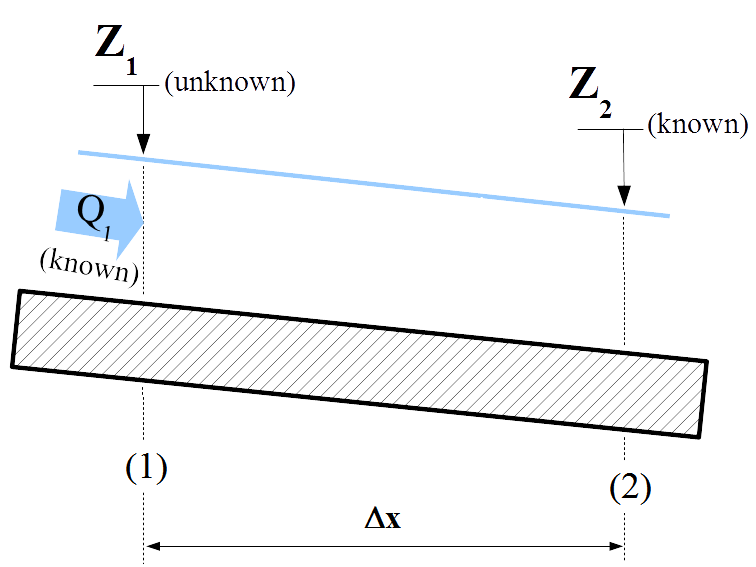
\includegraphics[width=\textwidth]{Figures/Principe_Res_Perm.png}
  \caption{Principle of the steady flow solution}
  \label{fig:PRP}
 \end{center}
\end{figure}

The equation of the water line is discretised between sections 1 and 2 in the following form :

\begin{eqnarray}
  \frac{q_l}{2 g} \left ( \beta_1 \frac{V_1}{S_1} + \beta_2 \frac{V_2}{S_2} \right ) + \frac{V_{1}^2+V_{2}^2}{4 g} \frac{\beta_2 - \beta_1}{\Delta x} + \frac{Z_2-Z_1}{\Delta x} + \nonumber \\
  \frac{1}{\Delta x} \left ( \beta_2 \frac{V_{2}^2}{2 g} - \beta_1 \frac{V_{1}^2}{2 g}  \right ) + \frac{2}{\displaystyle \frac{1}{J_1}+\frac{1}{J_2}} + \nonumber \\
  \frac{\zeta_1}{\Delta x} \frac{\left ( \beta_1 V_1 - \beta_2 V_2 \right ) ^2 }{2 g} + \frac{\zeta_2}{\Delta x} \beta_1 \frac{V_{1}^2}{2 g} = 0
  \label{Dyn5}
\end{eqnarray}

It can also be written :

\begin{equation}
  Z_1 = Z_2 + JDX + JSDX + DXBETA + DXQ + DXV
\end{equation}
where :
\begin{equation}
  JDX = \frac{2}{\displaystyle \frac{1}{J_1} + \frac{1}{J_2}} \Delta x
\end{equation}

\begin{equation}
  JSDX = \frac{1}{2 g} \left ( \zeta_1 \left ( B_1 V_1 - B_2 V_2 \right )^2 + \zeta_2 B_1 V_{1}^2 \right )
\end{equation}

\begin{equation}
  DXBETA = \frac{1}{2 g}(\beta_2 - \beta_1) \left ( \frac{V_{1}^2 + V_{2}^2}{2} \right )
\end{equation}

\begin{equation}
  DXQ = \frac{1}{2 g}(Q_2 - Q_1) \left ( \frac{\beta_1 V_1}{S_1} + \frac{\beta_2 V_2}{S_2} \right )
\end{equation}

and :

\begin{equation}
  DXV = \frac{1}{2 g} ( \beta_2 V_{2}^2 - \beta_1 V_{1}^2 )
\end{equation}

which is equivalent to :

\begin{equation}
  \label{ptfix}
  Z_1 = f(Z_1)
\end{equation}

We must therefore solve the equation (\ref{ptfix}) with the unknown $Z_1$ knowing that there are \textit{a priori} several solutions ; we seek the subcritical solution.

The method involves determining the roots of the function : $\varepsilon = Z_1 - f(Z_1)$.

We start with the approximated solution : $Z_1(0) = Z_2 + J_2 \Delta x$.

We calculate two other approximated solutions with the help of (\ref{ptfix}) : \\
$Z_1(1) = f(Z_2(0))$ hence : $\varepsilon_0 = Z_1(0) - Z_1(1)$ \\
$Z_1(2) = f(Z_1(1))$ hence : $\varepsilon_1 = Z_1(1) - Z_1(2)$

We therefore know two points, $A$ et $B$, of the function $\varepsilon$ (see figure \ref{fig:calsolapproc}) :

\begin{figure}[H]
 \begin{center}
  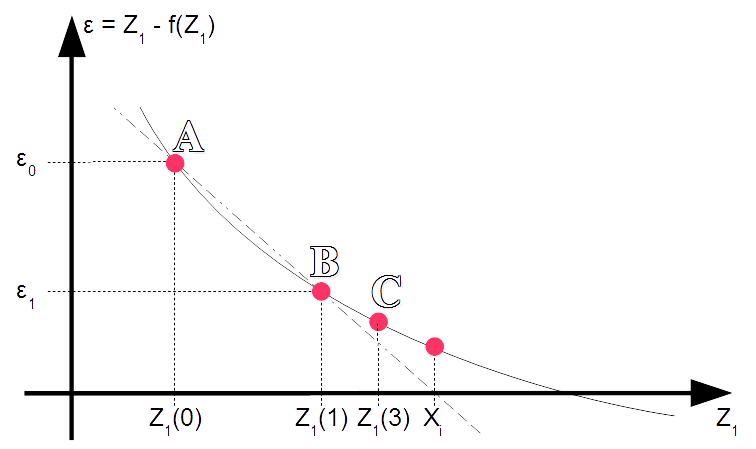
\includegraphics[width=\textwidth]{Figures/Princ_Cal_Sol_Apr.png}
  \caption{Calculation principle for the approximate solution}
  \label{fig:calsolapproc}
 \end{center}
\end{figure}

Knowing these two points, we can use the \textit{secant method} to calculate another approximated solution $X_i$. Experience shows that it is not desirable to use this value, but rather the half-sum of the solutions closest to the axis of $Z_1$, i.e. in figure \ref{fig:calsolapproc} : $Z_{1}(3) = \frac{X_i + Z_{1}(1)}{2}$.

We then calculate $\varepsilon(Z_{1}(3))$, which will give another point on the graph $\varepsilon(Z_1)$, the point $C$. The process resumes from the two points closest to the axis of $Z_1$ (in our case : $B$ et $C$).

We therefore proceed in an iterative manner.

In the case where $\varepsilon(Z_1)$ always keeps the same sign, we stop the calculation when the criteria  $\varepsilon(Z) \leq \Delta$ is satisfied by : $\Delta = 10^{-6}$.

In the case where $\varepsilon(Z)$ changes sign, we initially eliminate, from the two points that are on the same side of the axis of the $Z_1$, the point that is furthest away from it.  We then determine a new approximation from the half-sums of the remaining points.

The calculation is repeated until the stopping criterion is satisfied.

Comment on the solution obtained :
\begin{itemize}
 \item in general, the calculation converges within 10 iterations;
 \item the solution obtained is usually subcritical; however, the following paragraph explains the procedure adopted when this is not the case.
\end{itemize}

\begin{figure}[H]
 \begin{center}
  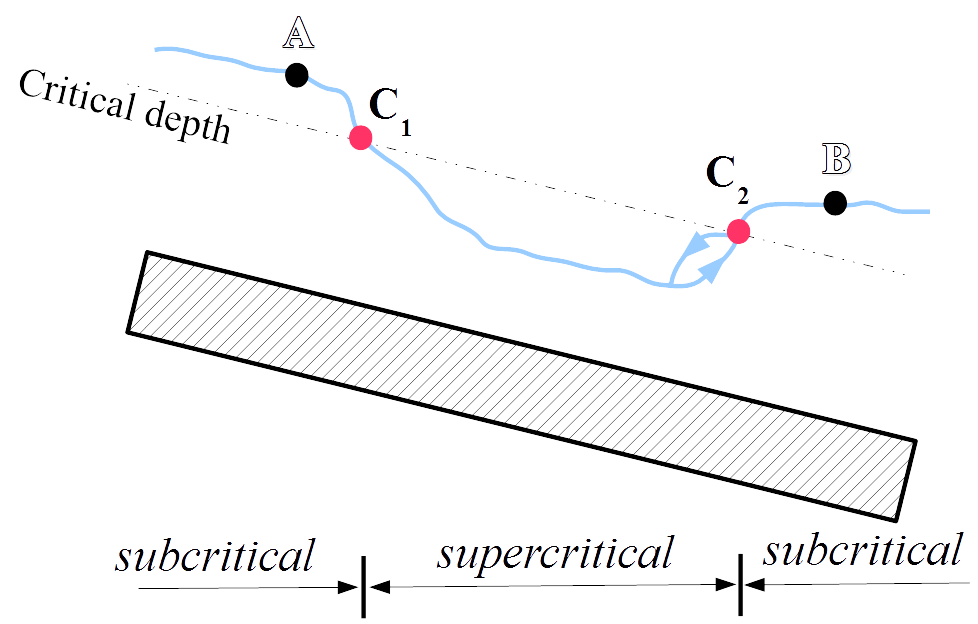
\includegraphics[width=\textwidth]{Figures/Pass_Loc_Tor.png}
  \caption{Diagram of a local passage in supercritical flow}
  \label{fig:PLT}
 \end{center}
\end{figure}


%...............................................................................
\subsubsection{Solving of supercritical zones}
%...............................................................................

When scanning up and down to calculate the subcritical zones, the supercritical zones are also detected (Figure \ref{fig:PLT}). In this case the domain will be swept from upstream to downstream and, for each supercritical zone, a finite-differences discretisation scheme will be applied.

The continuity equation has already been solved at the time of sweeping downstream to upstream. The discharge is known in all points of the discretisation. The equation of the water line, discretised between the section 1 and 2, is similar to equation (\ref{Dyn5}). As opposed to the treatment of subcritical zones, $Z_1$ is known and we look for $Z_2$.

It can also be written :

\begin{equation}
  Z_2 = Z_1 - JDX - JSDX - DXBETA - DXQ - DXV
\end{equation}

As previously, we eventually have to solve the equation :
\begin{equation}
  \label{ptfix1}
  Z_2 = G(Z_2)
\end{equation}

We must therefore solve the equation (\ref{ptfix1}) of unknown $Z_2$ admitting \textit{a priori} several solutions ; we look for the supercritical solution.

The method involves determining the roots of the function : $\varepsilon = Z_2 - f(Z_2)$.
To do that, we do not use the tangent method because the convergence to the supercritical solution would not be assured. The method used is a dichotomy method from the critical level calculated at each point during the calculation of the subcritical zones. The step of the dichotomy is the lesser of :
\begin{itemize}
 \item a $one-hundredth$ of the difference between the elevation of the bottom and the critical water level
 \item and $0.01 m$.
\end{itemize}

The solution is supercritical by construction.

%...............................................................................
\subsubsection{Validity of the hydraulic jump using impulse functions}
%...............................................................................

Once the supercritical zone has been covered, we check that the hydraulic jump is possible from an energy point of view by considering the direction of the increase of the impulse function at the hydraulic jump. It is reminded that impulse functions are maintained through the passage of the hydraulic jump.

\begin{equation}
F_{imp} = \frac{Q^2}{S}+gSh_G \quad \mbox{with : }h_G=\frac{1}{S}\int_0^h(h-y)dy
\end{equation}

If the impulse function at the upstream of the hydraulic jump is higher than the impulse function downstream of the hydraulic jump, the hydraulic jump is moved backward and the flow remains supercritical.

%...............................................................................
\subsection{Unsteady flow in a reach}
%...............................................................................

%...............................................................................
\subsubsection{Principle}
%...............................................................................

We consider the most general case of a compound channel consisting of : low flow channel, high flow channel and storage areas. We consider first the resolution for an unsteady flow for a single reach; the case of branched and meshed networks (possible with the unsteady flow engine) is considered in section \ref{NDRezo}.

We recall the equations governing the water line :
\begin{itemize}
 \item Continuity equation :
   \begin{equation}
     \frac{\partial Q}{\partial x} + L_t \frac{\partial Z}{\partial t} = q_l
   \end{equation}
   where $L_t$ is the total surface width, including the width of the low flow and high flow channels and the storage areas.
  \item Dynamic equation :
    \begin{equation}
      \label{qmv2}
      \frac{\partial Q}{\partial t} + \frac{\partial \beta Q V}{\partial x} + g S \left( \frac{\partial Z}{\partial x} + J + J_s\right) = 0
    \end{equation}
\end{itemize}

This equation (\ref{qmv2}) can also be written by involving the conveyance $D$ :

\begin{equation}
  Q |Q| + D^2 \left ( \frac{\partial Z}{\partial x} +J_s + \frac{1}{S g} \left ( \frac{\partial Q}{\partial t} + \frac{\partial \beta Q V}{\partial x}\right ) \right ) = 0
\end{equation}

These equations are solved with a finite-difference method (see figure \ref{fig:DF}), using an implicit scheme. The discretisation is of the Wendroff type, $\theta$ is the coefficient of implicitation. In a subcritical regime, the scheme is stable when : $\theta > 0.5$ (see \cite{CUNGE64}).

\begin{figure}[H]
 \begin{center}
  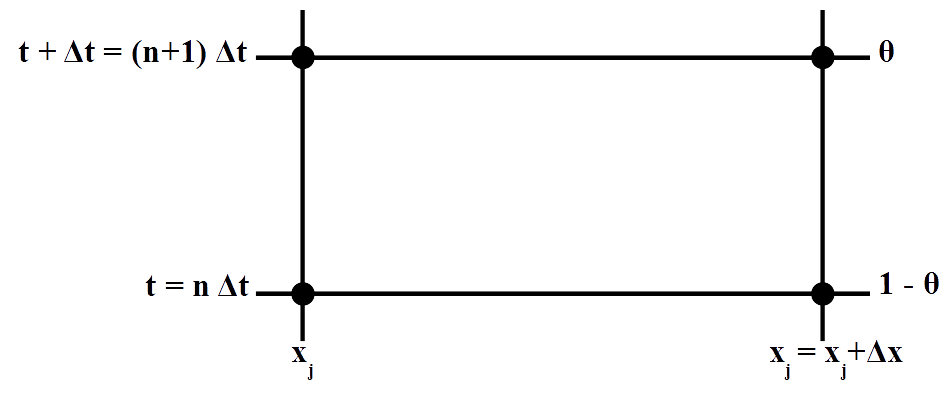
\includegraphics[width=\textwidth]{Figures/Disc_DF.png}
  \caption{Finite differences discretisation}
  \label{fig:DF}
 \end{center}
\end{figure}

We recall the convention : $i = j + 1$. To be rigorous, $\Delta x$ should be written as $\Delta x_j$, the spatial step varying \textit{a priori} in the considered reach.

The derivatives with respect to $x$ and $t$ are calculated (in the first order) in the following way :

\begin{equation}
  \frac{\partial f}{\partial x} = \theta \frac{f_{i}^{n+1}-f_{j}^{n+1}}{\Delta x} + (1-\theta) \frac{f_{i}^n - f_{j}^n}{\Delta x}
\end{equation}

\begin{equation}
  \frac{\partial f}{\partial t} = \frac{1}{2} \left ( \frac{f_{i}^{n+1} - f_{i}^n}{\Delta t} + \frac{f_{j}^{n+1} - f_{j}^n}{\Delta t} \right )
\end{equation}

The functions that occur without a derivative are evaluated by :

\begin{equation}
  f = \theta \frac{f_{i}^{n+1} + f_{j}^{n+1}}{2} + (1 - \theta) \frac{f_{i}^n + f_{j}^n}{2}
\end{equation}

%...............................................................................
\subsubsection{Discretised equations}
%...............................................................................

The discretised equations are written as follows :

\begin{itemize}
  \item Continuity equation :
  \begin{eqnarray}
    (1 - \theta) \frac{Q_{i}^n - Q_{j}^n}{\Delta x} + \theta \frac{Q_{i}^{n+1} - Q_{j}^{n+1}}{\Delta x} + \frac{1}{2} \left ( L_{t_i}^n + L_{t_j}^n \right ) \nonumber \\
    \times \frac{1}{2} \left ( \frac{Z_{i}^{n+1} - Z_{i}^n}{\Delta t} + \frac{Z_{j}^{n+1} - Z_{j}^n}{\Delta t} \right ) = q_{l_j}^{n+1}
  \end{eqnarray}

  \item Dynamic equation :
  \begin{eqnarray}
    \left ( \frac{1 - \theta }{2} \right ) \left ( Q_{j}^{n^2} + Q_{i}^{n^2} \right ) + \frac{\theta}{2} \left ( Q_{j}^{n+1^2} + Q_{i}^{n+1^2} \right ) \nonumber \\
    + \left ( \frac{1 - \theta}{2} \left ( D_{i}^{n^2} + D_{j}^{n^2} \right ) + \frac{\theta}{2} \left ( D_{i}^{n^2} + D_{j}^{n+1^2} \right ) \right ) \nonumber \\
    \times \Bigg \{ (1 - \theta) \frac{Z_{i}^n - Z_{j}^n}{\Delta x} + \theta \frac{Z_{i}^{n+1} - Z_{j}^{n+1}}{\Delta x} + J_{s}(i) + J_{s}(j) \nonumber \\
    + \left ( \frac{1 - \theta}{2 g} \left ( \left ( \frac{1}{S} \right )_{i}^n + \left ( \frac{1}{S} \right )_{j}^n \right ) + \frac{\theta}{2 g} \left ( \left ( \frac{1}{S} \right )_{i}^{n+1} + \left ( \frac{1}{S} \right )_{j}^{n+1} \right ) \right ) \nonumber \\
    \times \Bigg [ \frac{1}{2 \Delta t}(Q_{i}^{n+1}-Q_{i}^n+Q_{j}^{n+1}-Q_{j}^n) + \frac{\theta}{\Delta x} \left ( \beta_{i}^n \frac{Q_{i}^{n+1^2}}{S_{i}^{n+1}}-\beta_{j}^n \frac{Q_{j}^{n+1^2}}{S_{j}^{n+1}} \right ) \nonumber \\
    + \frac{1-\theta}{\Delta x} \left ( \beta_{i}^n \frac{Q_{i}^{n^2}}{S_{i}^{n}}-\beta_{j}^n \frac{Q_{j}^{n^2}}{S_{j}^{n}} \right ) \Bigg ] \Bigg \} = 0
  \end{eqnarray}
\end{itemize}

We introduce the following variables :

\begin{equation}
 \left \lbrace
  \begin{array}{l}
    \Delta Q_j = Q_{j}^{n+1} - Q_{j}^n \\
    \Delta Q_i = Q_{i}^{n+1} - Q_{i}^n \\
    \Delta Z_j = Z_{j}^{n+1} - Z_{j}^n \\
    \Delta Z_i = Z_{i}^{n+1} - Z_{i}^n
  \end{array}
 \right.
\end{equation}

and, after linearisation (i.e. preserving only the first order terms in $\Delta Z$ and $\Delta Q$) we get :

\begin{itemize}
 \item for the continuity equation :
  \begin{equation}
   \label{CONT}
   \boxed{
     G \Delta Q_i + H \Delta Z_i = I \Delta Q_j + J \Delta Z_j + K
   }
  \end{equation}
  with :
  \begin{equation}
   \label{CONT1}
   G = \theta
  \end{equation}
  \begin{equation}
    \label{CONT2}
   I = G
  \end{equation}
  \begin{equation}
    \label{CONT3}
   H = \frac{\Delta x}{4 \Delta t} ( L_{t_j}^n + L_{t_i}^n )
  \end{equation}
  \begin{equation}
    \label{CONT4}
   J = -H
  \end{equation}
   \begin{equation}
   \label{CONT5}
   K = Q_{j}^n - Q_{i}^n + q_{l_i}^{n+1}
  \end{equation}

 \item and for the dynamic equation :
  \begin{equation}
   \label{DYN}
   \boxed{
     L \Delta Q_i + M \Delta Z_i = N \Delta Q_j + O \Delta Z_j + P
   }
  \end{equation}
  with :
  \begin{equation}
    \label{DYN1}
   L = B_2 + C_1 H_1 ( E_2 + F_2 )
  \end{equation}
  \begin{equation}
    \label{DYN2}
   M = C_1 ( D_4 + H_1 F_4 + H_4 F_1 ) + C_4 ( D_1 + H_1 F_1 )
  \end{equation}
   \begin{equation}
    \label{DYN3}
   N = -B_3 - C_1 H_1 ( E_3 + F_3 )
  \end{equation}
  \begin{equation}
     \label{DYN4}
   O = -C_1 ( D_5 + H_1 F_5 + H_5 F_1 ) - C_5 ( D_1 + H_1 F_1 )
  \end{equation}
  \begin{equation}
   \label{DYN5}
   P = -B_1 - C_1 ( D_1 + H_1 F_1 )
  \end{equation}
\end{itemize}

knowing that the various terms of the dynamic equation have been linearised in the following way (the non-indexed variables correspond to the time steps $n$) :

\begin{equation}
 Q |Q| = B_1 + B_2 \Delta Q_i + B_3 \Delta Q_j
\end{equation}

\begin{equation}
 B_1 = \frac{1}{2} ( Q_{i}^2 sign(Q_i) + Q_{j}^2 sign(Q_j) )
\end{equation}

\begin{equation}
 B_2 = \theta |Q_i|
\end{equation}

\begin{equation}
 B_3 = \theta |Q_j|
\end{equation}

\begin{itemize}
 \item[*]
  \begin{equation}
   D^2 = C_1 + C_4 \Delta Z_i + C_5 \Delta Z_j
  \end{equation}
  \begin{equation}
   C_1 = \frac{1}{2} ( D_{i}^2 + D_{j}^2 )
  \end{equation}
  \begin{equation}
   C_4 = \theta D_i ( \alpha_{m_i} + \alpha_{M_i} )
  \end{equation}
  \begin{equation}
   C_5 = \theta D_j ( \alpha_{m_j} + \alpha_{M_j} )
  \end{equation}
  \begin{equation}
   \alpha_{m_i} = \frac{K_m R_{m}^{2/3}}{3} \left ( 5 L_m -2 R_m \frac{\partial P_m}{\partial z} \right )_i
  \end{equation}
   \begin{equation}
   \alpha_{m_j} = \frac{K_m R_{m}^{2/3}}{3} \left ( 5 L_m -2 R_m \frac{\partial P_m}{\partial z} \right )_j
  \end{equation}
  \begin{equation}
    \alpha_{M_i} = \frac{K_M R_{M}^{2/3}}{3} \left ( 5 L_M -2 R_M \frac{\partial P_M}{\partial z} \right )_i
  \end{equation}
  \begin{equation}
    \alpha_{M_j} = \frac{K_M R_{M}^{2/3}}{3} \left ( 5 L_M -2 R_M \frac{\partial P_M}{\partial z} \right )_j
  \end{equation}
  \begin{equation}
    K_{m}' = A K_m
  \end{equation}
  \begin{equation}
    K_{M}' = \sqrt{1 + \frac{S_m}{S_M} (1-A^2)} K_M
  \end{equation}
 \item[*]
  \begin{equation}
    \frac{\partial Z}{\partial x} + J_{s}(i) + J_{s}(j) = D_1 + D_4 \Delta Z_i + D_5 \Delta Z_j
  \end{equation}
  \begin{equation}
     D_1 = \frac{Z_i - Z_j}{\Delta x} + J_{s}(i) + J_{s}(j)
  \end{equation}
  \begin{equation}
    D_4 = \frac{\theta}{\Delta x}
  \end{equation}
    \begin{equation}
    D_5 = \frac{\theta}{\Delta x}
  \end{equation}
 \item[*]
   \begin{equation}
     \frac{\partial Q}{\partial t} = E_2 \Delta Q_i + E_3 \Delta Q_j
   \end{equation}
   \begin{equation}
     E_2 = \frac{1}{2 \Delta t}
   \end{equation}
   \begin{equation}
     E_3 = \frac{1}{2 \Delta t}
   \end{equation}
 \item[*]
   \begin{equation}
    \frac{\partial}{\partial x} \left ( \beta \frac{Q^2}{S} \right ) = F_1 + F_2 \Delta Q_i + F_3 \Delta Q_j + F_4 \Delta Z_i + F_5 \Delta Z_j
   \end{equation}
   \begin{equation}
     F_1 = \frac{1}{\Delta x} ( \beta_i V_i Q_i - \beta_j V_j Q_j )
   \end{equation}
   \begin{equation}
     F_2 = \frac{2 \theta}{\Delta x} \beta_i V_i
   \end{equation}
   \begin{equation}
     F_3 = -\frac{2 \theta}{\Delta x} \beta_j V_j
   \end{equation}
   \begin{equation}
     F_4 = - \frac{\theta}{\Delta x} \beta_i V_{i}^2 L_{t_i}
   \end{equation}
   \begin{equation}
     F_5 = \frac{\theta}{\Delta x} \beta_j V_{j^2} L_{t_j}
   \end{equation}
 \item[*]
   \begin{equation}
    \frac{1}{S g} = H_1 + H_4 \Delta Z_i + H_5 \Delta Z_j
   \end{equation}
   \begin{equation}
     H_1 = \frac{1}{2 g} \left ( \frac{1}{S_i} + \frac{1}{S_j} \right )
   \end{equation}
   \begin{equation}
     H_4 = - \frac{\theta}{2 g} \frac{L_{t_i}}{S_{i}^2}
   \end{equation}
   \begin{equation}
     H_5 = - \frac{\theta}{2 g} \frac{L_{t_j}}{S_{j}^2}
   \end{equation}
\end{itemize}

%...............................................................................
\subsubsection{Solving the discretised equations}
%...............................................................................

The equations (\ref{CONT}) and (\ref{DYN}) lead directly to the establishment of a matrix system :

\begin{equation}
 \label{systm}
 \left(
    \begin{array}{cc}
       G & H \\
       L & M
    \end{array}
 \right)
 \left(
    \begin{array}{c}
       \Delta Q_i \\
       \Delta Z_i
    \end{array}
 \right)
 =
  \left(
    \begin{array}{cc}
       I & J \\
       N & O
    \end{array}
 \right)
 \left(
    \begin{array}{c}
       \Delta Q_j \\
       \Delta Z_j
    \end{array}
 \right)
 +
 \left(
    \begin{array}{c}
       K \\
       P
    \end{array}
 \right)
\end{equation}

where $G$,$H$,$I$,$J$,$K$,$L$,$M$,$N$,$O$ et $P$ are macro-coefficients, their expression
depend on the control variables, the state variables and the parameters of the model (\ref{CONT1}-\ref{CONT5}) (\ref{DYN1}-\ref{DYN5}).

In the case of a single reach, the boundary conditions at the upstream and downstream ends mean that $\Delta Q_1$ and $\Delta Z_n$ are no longer unknowns, $n$ being the number of calculation sections. This corresponds to an imposed discharge at the upstream end and an imposed water level at the downstream end. The system (\ref{systm}) therefore comprises $2n-2$ equations and as many unknowns. It is expressed in the general form :

\begin{equation}
 \label{eq1}
 A.x = b
\end{equation}
where :
\begin{itemize}
 \item the vector $x$ of the unknowns, is the solution of the variations of elevation and discharge at each one of the $n$ calculation sections in the network of reaches :
   \begin{equation}
      x = \left(
            \begin{array}{c}
               \Delta Z_1\\
               \Delta Q_2\\
               \Delta Z_2\\
               \Delta Q_3\\
               \Delta Z_3\\
               \vdots\\
               \Delta Z_{n-1}\\
               \Delta Q_{n}
            \end{array}
          \right)
   \end{equation}
 \item in the simple case of a single reach, the matrix $A$ is an asymmetric band matrix :
   \begin{equation}
     \label{eq3}
     A = \left(
         \begin{array}{cccccccccccc}
          -J & G & H & & & & & & & & & \\
          -O & L & M & & & & & & & & & \\
             & -I & -J & G & H & & & & & & & \\
             & -N & -O & L & M & & & &  & 0 & & \\
             & & & -I & -J & G & H & & & & & \\
             & & & -N & -O & L & M & & & & & \\
             & & & & & & & .... & & & & \\
             & & & & & & & & .... & & & \\
             & 0 & & & & & & & & .... & & \\
             & & & & & & & & & & .... & \\
             & & & & & & & & & -I & -J & G \\
             & & & & & & & & & -N & -O & L \\
         \end{array}
         \right)
   \end{equation}
 \item $b$ is the vector of the second member of the equation :
   \begin{equation}
      \label{eq2}
      b = \left(
            \begin{array}{c}
               K\\
               P\\
               K\\
               P\\
               \vdots\\
               K\\
               P
            \end{array}
          \right)
   \end{equation}
\end{itemize}

The various macro-coefficients $G, H, I, J, K, L, M, N, O\ et\ P$ are calculated at each time step.

The matrix $A$ presents two important characteristics : it is a diagonally-dominant band matrix and is very sparse. It is then possible to use a specialised solver to solve (\ref{eq1}).

Two linear solvers are implemented in the code \REZO{}.

\begin{itemize}
  \item the first one is the band solver \texttt{DGBSV} of the \texttt{LAPACK}\footnote{http://www.netlib.org/lapack/} numerical library. This solver is the default one when the problem deals with only one reach with no storage cell;
  \item the second is a sparse solver written in %\textit{Fortran77} \texttt{Y12M}\footnote{http://www.netlib.org/y12m/}. This program was developed at %the beginning of the 1980s \cite{ZLATEV81}. It benefits from a robustness and performance proven for %the size of problems that the code \REZO{} is used for.\texttt{Y12M} is a direct solver with numerical pivoting to preserve the stability of the calculation, and the sparseness of the matrix factorised as an $L.U$ product. Using this solver is particularly simple and light because of :
\begin{itemize}
 \item the call of a single routine and a reduced number of sources;
 \item the internal management of the renumbering to preserve the sparseness (a choice of the pivot, with a criterion of fill minimization);
 \item the matrix chaining is filled using the coordinates format $(i,j)$ for each non-zero element that is present in the line $i$ and column $j$.
\end{itemize}

\end{itemize}

The solving of a sub-critical and unsteady problem by the \REZO{} code follows the algorithmic stages described in Figure \ref{fig:Etap}.

\begin{figure}[H]
 \begin{center}
  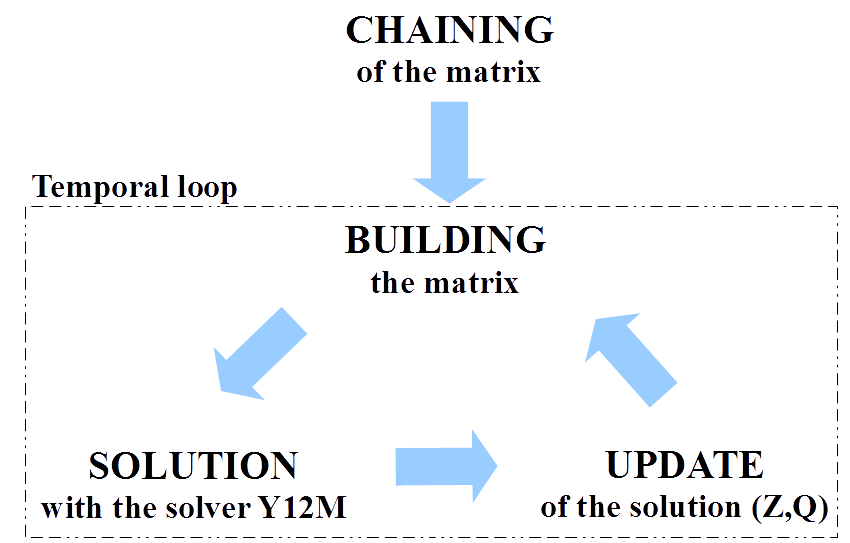
\includegraphics[width=0.8\textwidth]{Figures/AlgoRezo.png}
  \caption{\REZO{} algorithm}
  \label{fig:Etap}
 \end{center}
\end{figure}

Before starting the time-based simulation, the chaining of the matrix must be determined, starting with the schematic of the network. This calculation is carried out only once because the connectivity of the network does not change with time.

The time loop consists of three phases :
\begin{itemize}
 \item a calculation of the macro-coefficients $G, H, I, J, K, L, M, N, O\ and\ P$ and their assembly in the matrix $A$ and the second member of the equation $b$;
 \item the use of the direct solver \texttt{Y12M} or \texttt{DGBSV }for solving the system (\ref{eq1}) and determine the solution of the elevation and discharge variations $(\Delta Z_i,\Delta Q_i)$ in each section $i$;
 \item an update of the water line for the current time $t_k$ :
  \begin{equation}
   \forall i \in 1...n
   \left \lbrace
  \begin{array}{l}
    Q_{i}^{k} = Q_{i}^{k-1} + \Delta Q_i \\
    \\
    Z_{i}^{k} = Z_{i}^{k-1} + \Delta Z_i
  \end{array}
 \right.
  \end{equation}
\end{itemize}

%...............................................................................
\subsection{Treatment of junctions in a steady subcritical regime} \label{NdPERM}
%...............................................................................

%...............................................................................
\subsubsection{Reminder}
%...............................................................................

The equations solved at the junctions are :
\begin{itemize}
 \item the continuity of discharges;
 \item the equality of elevations in each branch (see the justification in section \ref{TrNd}).
\end{itemize}

Therefore a junction does not add any additional unknown : the unknowns to be calculated are the unknowns $(Z,Q)$ of the computational sections forming this junction. Therefore, in the example below (figure \ref{fig:SchNd}):

\begin{figure}[H]
 \begin{center}
  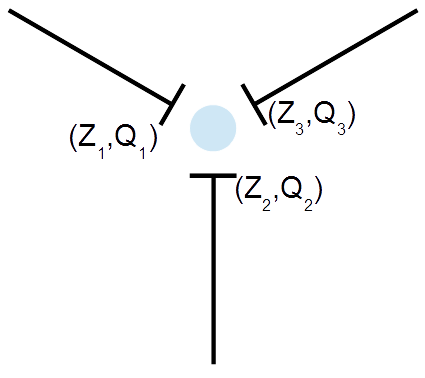
\includegraphics[width=0.8\textwidth]{Figures/Schema_noeud.png}
  \caption{Example of a junction with three branches}
  \label{fig:SchNd}
 \end{center}
\end{figure}

The unknowns are $(Z_1,Q_1)$, $(Z_2,Q_2)$ and $(Z_3,Q_3)$ and the equations of the junction are :
\begin{itemize}
 \item the distribution of discharges : $Q_1 + Q_2 + Q_3 = 0$;
 \item the equality of the water levels : $Z_1 = Z_2 = Z_3$.
\end{itemize}

We can easily verify that these relationships are sufficient to determine the values of $(Z,Q)$ throughout the considered network.

If we call :
\begin{itemize}
 \item the total number of computational sections to be processed (i.e. the sum of the calculation sections in all of the branches) : $im$;
 \item the number of reaches : $nbreach$;
 \item the number of free ends : $nblimi$.
\end{itemize}

then for the whole network we can write $(im-nbreach)$ continuity equations and as many discrete dynamic equations of Saint-Venant.

The unknowns are the $(\Delta Q,\Delta Z)$ of the computation sections, and so there are $2 im$ unknowns.

The boundary conditions are known at the extremities, which gives $nblimi$ additional relationships.

For all of the nodes we can write :
\begin{itemize}
 \item[*] $nbnode$ discharge conservation equations;
 \item[*] $(2nbreach-nblimi) - nbnode$ equal elevation equations.
\end{itemize}

This is because $(2nbreach - nblimi)$ represents the number of branch extremities connecting to a junction (each reach should be counted twice except those that have a free end). At each junction, if $k$ branches are connected, there are only $k-1$ equations that come from the equality of elevations. It is therefore necessary to subtract $nbnode$ from $2nbreach - nblimi$.

Finally, we have : \\
$2 (im - nbreach) + nblimi + nbnode + (2 nbreach - nblimi) - nbnode$
$= 2 im$ equations for $2 im$ unknowns.

%...............................................................................
\subsubsection{Principle}
%...............................................................................

The algorithm presented here is valid regardless of the network (branched or meshed) provided the following conditions are met :
\begin{itemize}
 \item the direction of flow is known \textit{a priori} in each reach;
 \item for all extremities, the boundary condition is:
   \begin{itemize}
     \item the discharge, if it is an upstream end;
     \item the elevation, if it is a downstream end.
    \end{itemize}
\end{itemize}

In practice, there is a risk that this algorithm becomes very time consuming if the network is complex (i.e. interconnected distributaries, see below). In that case, it would be better to use the unsteady subcritical engine (see the following section), starting with a simple initial water line, and choosing the boundary conditions so as to converge towards a stationary state corresponding to the water line being sought.

Before presenting the algorithm, it is useful to make the following observation. The problem is very simple if the network is only comprised of confluences because the discharge is calculated at every point of the domain descending from the upstream ends ; therefore it suffices to calculate the elevation of the water line by following the reverse path (i.e. gradually moving towards the upstream ends), using the same procedure as for a reach. At each node, the equality of the elevations can be imposed without difficulty.

The critical problem is therefore to calculate the distribution of discharge at a junction. The solution used here is an iterative method that is explained in the following paragraph. This means that the general algorithm is itself iterative : the iterations are interlinked in the same way as the distributaries (see figures \ref{fig:AlgSP} and \ref{fig:ExSP}). We can further specify that :
\begin{itemize}
 \item \textit{to descend a reach} means to calculate the discharge at each successive computational section, working from upstream to downstream;
 \item \textit{to ascend a reach} means to calculate the elevation at each successive computational section, working from downstream to upstream.
\end{itemize}

Figure \ref{fig:AlgSP} presents the solution algorithm, while figure \ref{fig:ExSP} illustrates the example of a meshed network including two interlinked distributaries. This example could be considered as representative of the more complex cases that can be computed within a reasonable time by this algorithm. Beyond that, as indicated previously, it is recommended that the \REZO{} code for unsteady flows is used.

\begin{figure}[H]
 \begin{center}
  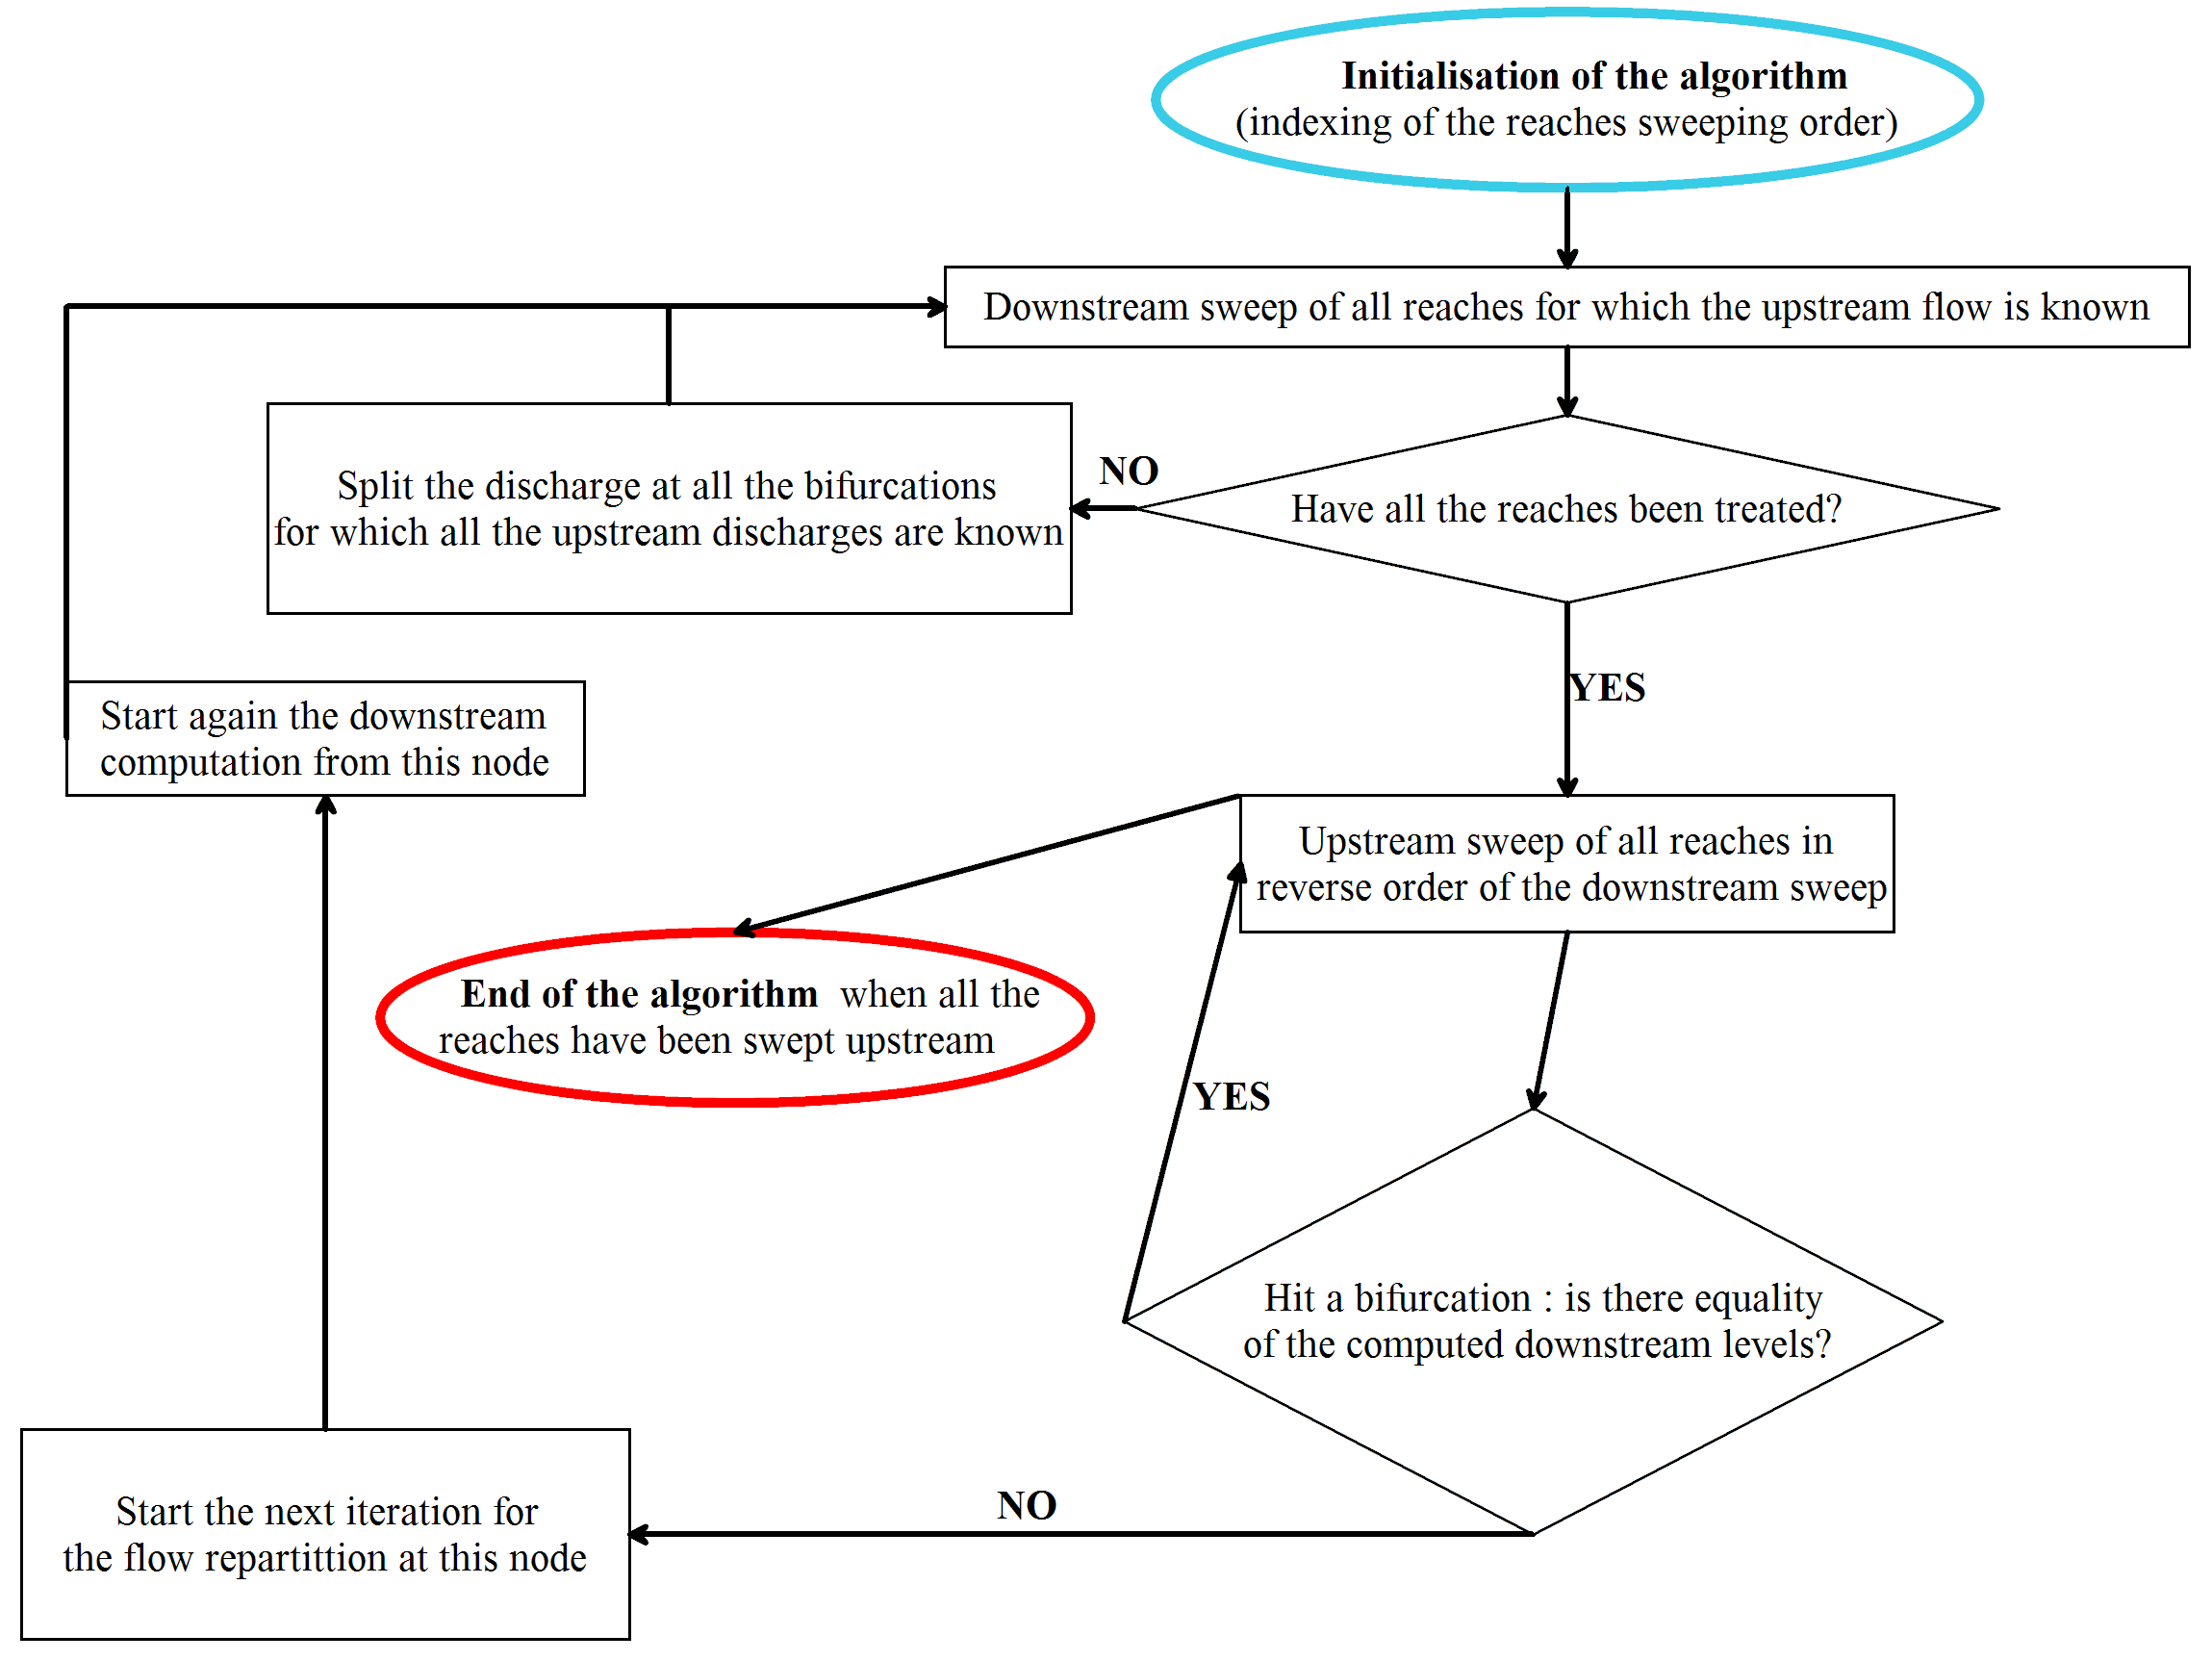
\includegraphics[width=\textwidth]{Figures/Algorithm_SARAP.png}
  \caption{Solution algorithm for a steady state network}
  \label{fig:AlgSP}
 \end{center}
\end{figure}

\begin{figure}[H]
 \begin{center}
  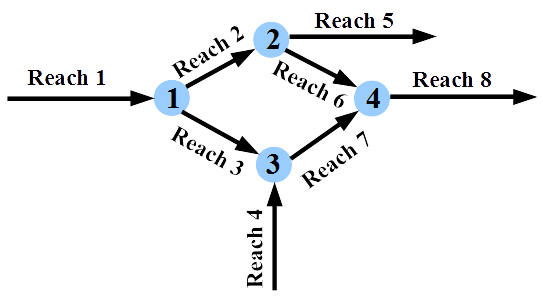
\includegraphics[width=\textwidth]{Figures/Ex_Res_SARAP.png}
  \caption{Example of a network for a steady state calculation}
  \label{fig:ExSP}
 \end{center}
\end{figure}

\textsc{\textbf{algorithm} (see figure \ref{fig:ExSP}) :}
\begin{itemize}
 \item[*] Descend Reach 1
 \item[*] Descend Reach 4
 \item[*] $n = 1$
 \item[*] \textbf{(1)} Spread the discharge at node 1 (iteration $n$)
 \begin{itemize}
  \item Descend Reach 2
  \item Descend Reach 3
  \item Descend Reach 7
  \item $p = 1$
  \item \textbf{(2)} Spread the discharge at node 2 (iteration $n.p$)
  \begin{itemize}
   \item Descend Reach 5
   \item Descend Reach 6
   \item Descend Reach 8
  \end{itemize}
  -----------------------------
  \begin{itemize}
   \item Ascend Reach 8
   \item Ascend Reach 6
   \item Ascend Reach 5
   \item Equality of the downstream elevations at node 2?
   \begin{itemize}
    \item if no : $p = p + 1$, go back to step \textbf{(2)}
    \item if yes : continue
   \end{itemize}
  \end{itemize}
  \item Ascend Reach 7
  \item Ascend Reach 3
  \item Ascend Reach 2
  \item Equality of the downstream elevations at node 1?
  \begin{itemize}
    \item if no : $n = n + 1$, go back to step \textbf{(1)}
    \item if yes : continue
   \end{itemize}
  \end{itemize}
 \item Ascend Reach 4
 \item Ascend Reach 1
\end{itemize}

%...............................................................................
\subsubsection{Discharge distribution in a diffluence (bifurcation)}
%...............................................................................

\textbf{First Iteration}

The discharge distribution needs to verify :

\begin{equation}
  Q_{us} + \sum_{i=1}^{n_{ds}} Q_i
\end{equation}
where $n_{ds}$ is the number of downstream branches.

\begin{equation}
  Q_i = D_i J_{i}^{1/2}
\end{equation}

The solution used here is the equality of the slopes of the total head line :

\begin{equation}
  J_i = J = \left ( \frac{Q_i}{D_i}^2 \right )
\end{equation}

or :

\begin{equation}
  \frac{Q_i}{D_i} = \frac{Q_j}{D_j} = ct = J^{1/2}
\end{equation}

Substituting this into the continuity equations leads to:

\begin{equation}
 \frac{Q_{us}}{J^{1/2}} = \sum_{i=1}^{n_{ds}} D_i
\end{equation}

The sum of the conveyances depends only on the geometry and the roughness of the downstream reaches and is a function of the elevation that, in general, increases monotonously.

For a given value of $J$, it is possible to calculate an elevation satisfying this relationship, and then calculate the $D_j$ and then the  $Q_j$ for that elevation.

In the current version of \mascaret{}, the approach used for the first iteration is to take $J$ as the average of the slopes of the bottom of the downstream branches.

\textbf{Subsequent iterations}

The problem to solve is determining the best corrections of discharge to make (compared to the distribution chosen for the previous iteration), in order to come as close as possible to the equality of elevations at the first sections of the downstream reaches.

The approach is to determine the correction of discharge by assuming the slopes of the energy lines $J$ (equal to those of the preceding iteration) in order to tend towards the equality of the elevations (while still respecting the continuity of the discharges).

For each of the first sections of the downstream branches, we can write (for a given elevation) :

\begin{equation}
 Q_{i}^2 = J_i D_{i}^2
\end{equation}
or :
\begin{equation}
 Q_{i} = J_{i}^{1/2} D_{i}
\end{equation}
the index $i$ corresponds to the number of the downstream branch.

By differentiating between the iterations $n$ and $n+1$, we get :
%and by developing the term $J_{i}^{1/2}$

\begin{equation}
 \label{i1}
 \delta Q_i = ( J_{i}^{1/2} )_n \left ( \frac{\partial D_i}{\partial Z_i} \right )_n \delta Z_i
\end{equation}
where $n$ denotes the number of the current iteration,

with :

\begin{equation}
 ( J_{i}^{1/2} )_n = \left ( \frac{Q_i}{D_i} \right )_n
\end{equation}

where : $\delta Q_i = Q_{i}^{n+1} - Q_{i}^{n}$
and : $\delta Z_i = Z_{i}^{n+1} - Z_{i}^{n}$

If $n_{ds}$ is the number of downstream branches then the continuity of the discharges is written  :
\begin{equation}
  Q_{us} = \sum_{i=1}^{n_{ds}} Q_i
\end{equation}
where :

\begin{equation}
 \label{i2}
 \sum_{i=1}^{n_{ds}} \delta Q_i = 0
\end{equation}

The correction of discharge is done to tend towards the equality of the elevations at the junction. We therefore want :

\begin{equation}
 Z_{i}^{n+1} = ct = Z
\end{equation}
which gives :

\begin{equation}
 \label{i3}
  \delta Z_i = Z - Z_{i}^n
\end{equation}
where the $Z_{i}^n$ are the results of the previous iteration.

So we have :
\begin{itemize}
 \item $n_{ds}$ relationships (\ref{i1});
 \item 1 relationship (\ref{i2});
 \item $n_{ds}$ relationships (\ref{i3}).
\end{itemize}
and so there are $2n_{ds}+1$ relationships for $2n_{ds}+1$ unknowns ($\delta Q_i$,$\delta Z_i$ and $Z$).

\begin{equation}
 \left \lbrace
  \begin{array}{l}
    \delta Z_i = Z - Z_{i}^n \\
    \sum_{i=1}^{n_{ds}} \delta Q_i = 0 \\
    \delta Q_i = \left ( \frac{Q_i}{D_i} \right )_n \left ( \frac{\partial D_i}{\partial Z_i} \right )_n \delta Z_i
  \end{array}
 \right.
\end{equation}

from which it can be derived :

\begin{equation}
  Z = \frac{\displaystyle \sum_{i=1}^{n_{ds}} \left ( \frac{Q_i}{D_i} \right )_n \left ( \frac{\partial D_i}{\partial Z_i} \right )_n Z_i}{\displaystyle \sum_{i=1}^{n_{ds}} \left ( \frac{Q_i}{D_i} \right )_n \left ( \frac{\partial D_i}{\partial Z_i} \right )_n}
\end{equation}
then :
\begin{equation}
  \delta Z_i = Z - Z_{i}^n
\end{equation}
and finally :
\begin{equation}
  \delta Q_i = \sum_{i=1}^{n_{ds}} \left ( \frac{Q_i}{D_i} \right )_n \left ( \frac{\partial D_i}{\partial Z_i} \right )_n \delta Z_i
\end{equation}


%...............................................................................
\subsection{Computation of junctions in unsteady subcritical flow} \label{NDRezo}
%...............................................................................

The matrix $A$ (\ref{eq3}) describes a solution to the 1D Saint-Venant equations in the case of a single reach. If several reaches exist, the representation of the confluents or diffluents requires additional equations. There are no dynamic equations (\ref{qmv}) or continuity equations (\ref{masse}) between the sections relating to the same junction (Figure \ref{fig:SchemConf}). For each subcritical junction of the network, it is necessary to take into account the two following constraints :

\begin{itemize}
 \item \underline{equality of the elevations} of each section of the reach extremities that are connected to the same node. In the case of a node of three branches (Figure \ref{fig:SchemConf}), it is necessary to add two equations involving the equality of the elevations from one time step to the next :
  \begin{equation}
    \left \lbrace
     \begin{array}{l}
       Z_1 + \Delta Z_1 = Z_2 + \Delta Z_2 \\
       Z_1 + \Delta Z_1 = Z_3 + \Delta Z_3
     \end{array}
    \right.
  \end{equation}
	which is rewritten as :
  \begin{equation}
    \left \lbrace
     \begin{array}{l}
       \Delta Z_1 - \Delta Z_2 = Z_2 - Z_1\\
       \Delta Z_1 - \Delta Z_3 = Z_3 - Z_1
     \end{array}
    \right.
  \end{equation}
  It is therefore necessary to add to the matrix $A$ (\ref{eq3}) two rows of coefficients $+1$ and $-1$ on the level variations. The second member vector $b$ (\ref{eq2}) is supplemented with two differences of elevation.

  \item \underline{conservation of the discharges}, the total volume of water arriving in a node is equal to the volume of all the water leaving the node :
   \begin{equation}
     Q_1 + \Delta Q_1 + Q_2 + \Delta Q_2 = Q_3 + \Delta Q_3
   \end{equation}
   that is to say :
   \begin{equation}
     \Delta Q_1 + \Delta Q_2 - \Delta Q_3 = Q_3 -Q_2 - Q_1
   \end{equation}
   In the same way as above, the matrix $A$ is supplemented with a line of $+1$ and $-1$ coefficients.  We add to the second member an algebraic sum of the discharges of the attached sections.
\end{itemize}

An exploration of the network for the solution of the discretised equations is no longer appropriate. The solution algorithm is particularly complex and a linear solver system is used, in this case \texttt{Y12M} \cite{ZLATEV81}.

%...............................................................................
\subsection{Treatment of the singularities} \label{TS}
%...............................................................................

In section \ref{singu} we have defined the modelling principle for the singularities : they are supposed to be located between two sections of calculation $j$ and $i = j + 1$. The continuity equation is replaced by the equality of the discharges for these sections, and the dynamic equation is replaced by the law of singularity of the following form after being discretised :

\begin{equation}
  A_{sing} \Delta Q + B_{sing} \Delta Z_{us} + C_{sing} \Delta Z_{ds} = D_{sing}
\end{equation}

with :
\begin{equation}
 \mbox{si} \quad Q > 0 \quad \left \lbrace
     \begin{array}{l}
      Z_{us} = Z_j\\
      Z_{ds} = Z_i
     \end{array}
    \right.
\end{equation}
and :
\begin{equation}
 \mbox{si} \quad Q < 0 \quad \left \lbrace
     \begin{array}{l}
      Z_{us} = Z_i\\
      Z_{ds} = Z_j
     \end{array}
    \right.
\end{equation}

We note that $A_{sing}$ can be zero, but that $B_{sing}$ and $C_{sing}$ cannot be zero at the same time without the system being undefined.

\textbf{Examples :}
\begin{itemize}
 \item Weir following the general relation : $Q = f(Z_{us},Z_{ds})$;
 $$ A_{sing} = -1 \quad;\quad B_{sing} = + \frac{\partial f}{\partial Z_{us}} \quad;$$
 $$ C_{sing} = + \frac{\partial f}{\partial Z_{ds}} \quad;\quad D_{sing} = 0 $$
 \quad If this weir is under free flow, then : $C_{sing} = 0$
 \item Dam for which the retention equation : $Z_{us} = f(t)$ is known \textit{a priori};
 $$ A_{sing} = 0 \quad;\quad B_{sing} = 1 \quad;$$
 $$ C_{sing} = 0 \quad;\quad D_{sing} = f(t+\Delta t)-f(t)$$
\end{itemize}

%...............................................................................
\subsubsection{Solving for steady flow}
%...............................................................................

We must determine the water elevation upstream of the singularity, knowing the discharge and the elevation downstream. The solution is therefore always very simple. In several cases (e.g. weirs of general law, a regulation, a control section), the discretisation of the law of the singularity gives the result directly. If not, the only difficulty lies with the drowned/free flow coefficient, the value of which supposes that the level upstream of the calculated object is already known.
In that case, the upstream elevation is initially calculated by assuming a free flow regime, then, if this is not the case with the solution obtained, the upstream elevation is progressively increased until the free flow regime is verified. Note that for a weir, the head is the height above the weir for the upstream section.

%...............................................................................
\subsubsection{Solution for unsteady flow}
%...............................................................................

The continuity equation (\ref{CONT}) is reduced to the equality of the discharges upstream and downstream of the singularity, which implies :
\begin{equation}
  \left \lbrace
     \begin{array}{l}
      H = 0\\
      J = 0\\
      G = 1\\
      I = 1
     \end{array}
    \right.
\end{equation}

The dynamic equation (\ref{DYN}) is specific to each type of singularity.  Nevertheless, this equation is modified as follows :

\begin{equation}
  \left \lbrace
     \begin{array}{l}
      L = 0\\
      N = -A_{sing}\\
      O = -B_{sing}\\
      M = C_{sing}\\
      P = D_{sing}
     \end{array}
    \right.
\end{equation}

where the coefficients $A_{sing}$, $B_{sing}$, $C_{sing}$ and $D_{sing}$ depend mainly on the nature of the weir and the type of regime (drowned or free flow). They are calculated \textit{a priori} for each time step by external functions and are used for the creation of the matrix of coefficients $A$ (\ref{eq3}). The discharges calculated over the weirs by solving the equation (\ref{eq1}) are corrected later by these same functions.

%...............................................................................
\subsection{Dealing with the transcritical flows}
%...............................................................................

%...............................................................................
\subsubsection{Introduction}
%...............................................................................

Until the version $7.1.3$, flows with a Froude number greater than 1 stop the computation of the unsteady subcritcal kernel.

Since the version $7.1.4$, critcial and supercritical flows can be avoided so that the computation does not stop.
This possibility is based on a simplication in the governing momentum equations.

This simplification is often used in engineering shallow water flow modelling softwares using a Preissmann scheme.

It makes impossible to reproduce the supercritical flow conditions and wave speed estimates are incorrect for large Froude numbers. Even if the robustness is improved (no computation error) the user must aware of the problem of a simplified model.

This modification is a trick that remains a numerical option since the version $7.1.4$ of \mascaret{}

%...............................................................................
\subsubsection{Subcritical modelling}
%...............................................................................

Initially, the Preissmann scheme cannot deal with the shallow water equations when a critical condition occurs because of a ill-posed problem \cite{MESELHE97}.

At the subcritical-supercritical transition, the system is locally underdeterminated because of only one forward characteristic on the correponding cross-section. On the contrary at the supercritical-subcritical transition,
the system is overdeterminated because of three forward characteristics instead of two.

Some authors have proposed modifications of the Preissmann scheme in order to deal with supercritical flows with a small Froude number \cite{KUTIJA02}\cite{JOHNSON02}.

These modifications are not straightforward and cannot be competitive in comparison with more modern schemes based on the finite volume approach \cite{TORO01}.

%...............................................................................
\subsubsection{Modifying the momentum equation}
%...............................................................................

The goal of the modification (and that only concerns the code \REZO{}) is to avoid to deal with a critical condition when the water flow is speeding up.

Thereby this not exactly the equation (\ref{qmv}) that is solved with a consistent discresitation scheme but an altered form where the convection term is multiplied by a weighting coefficient $\alpha$.

\begin{equation}
 \frac{\partial}{\partial x}\left( {\beta \frac{Q^2}{S}} \right) \rightarrow \alpha \times \frac{\partial}{\partial x}\left( {\beta \frac{Q^2}{S}} \right)
\end{equation}

with : $\alpha \in \lbrack 0,1 \rbrack$

The selection of the value for the weighting coefficient $\alpha$ is based on a heuristic depending on the local Froude number. For small values of the Froude number, $\alpha$ is close to $1$ in order to exactly solve the momentum equation.

On the contrary, for a  Froude number close to 1, $\alpha$ tends to $0$ in order to gradually decrease the speed-up.

The chosen formula est a regular function \cite{GUINOT10} :

\begin{equation}
   \alpha = max(0,1-F_{r}^{2})
\end{equation}

The attenuation of the convection term begins early with this formula.

\begin{figure}[H]
 \begin{center}
  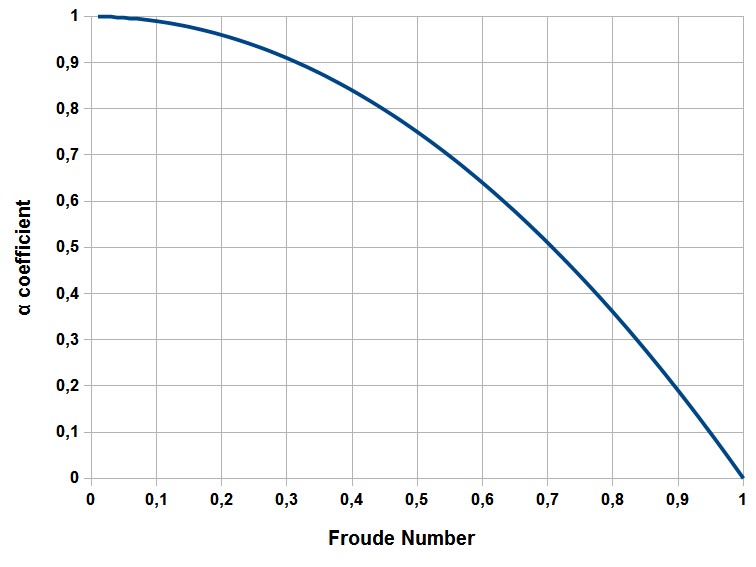
\includegraphics[width=0.8\textwidth]{Figures/Atten_Alpha.png}
  \caption{Coefficient $\alpha$ as a function of the Froude number}
 \end{center}
\end{figure}

With this simplification, the code \REZO{} is limited in its field of application: the subcritical flows.
This improves the robustness in various situations. In return, the fast phenomena are not represented. They are replaced by the calculation of a dummy water level that has no physical reality.
Therefore, the user must keep in mind the error committed by the code in rapid flow areas.
